\RequirePackage[l2tabu, orthodox]{nag}
\documentclass[10pt]{scrartcl}
% \documentclass[10pt]{article}
\usepackage[T1]{fontenc}
\usepackage{amsmath,amsfonts,amssymb}
\usepackage{mathtools}
\usepackage{color,soul}
\usepackage{fullpage}
\usepackage{enumerate}
\usepackage{graphicx}
\usepackage[colorlinks=true,urlcolor=blue]{hyperref}
\usepackage{caption}
\usepackage{subcaption}
\usepackage{floatrow}
\usepackage{deluxetable}
\usepackage{verbatim}
\usepackage{fancyvrb}
\usepackage{listings}
\usepackage{calc}
\usepackage[activate={true,nocompatibility},final,tracking=true,kerning=true,spacing=true,factor=1100,stretch=10,shrink=10]{microtype}

\floatsetup{ 
  heightadjust=object,
  valign=t
}

\definecolor{Light}{gray}{.90}
\sethlcolor{Light}

\lstset{%
language=IDL,                   % choose the language of the code
basicstyle=\footnotesize\sffamily,%\ttfamily\footnotesize,       % the size of the fonts that are used for the code
numbers=left,                   % where to put the line-numbers
numberstyle=\footnotesize,      % the size of the fonts that are used for the line-numbers
stepnumber=1,                   % the step between two line-numbers. If it is 1 each line will be numbered
numbersep=5pt,                  % how far the line-numbers are from the code
showspaces=false,               % show spaces adding particular underscores
showstringspaces=false,         % underline spaces within strings
showtabs=false,                 % show tabs within strings adding particular underscores
% frame=single,                   % adds a frame around the code
backgroundcolor=\color{Light},
columns=flexible,
tabsize=2,                      % sets default tabsize to 2 spaces
captionpos=b,                   % sets the caption-position to bottom
breaklines=true,                % sets automatic line breaking
breakatwhitespace=false,        % sets if automatic breaks should only happen at whitespace
escapeinside={\%*}{*)}          % if you want to add a comment within your code
}

\title{Some stuff about \#5}
\author{Jeren Suzuki}
\date{Last Edited \today}

\begin{document}

\maketitle
\pagenumbering{Roman}
% \tableofcontents
\clearpage
\pagenumbering{arabic}

\section{First set of 1D smoothing} % (fold)
\label{sec:First set of 1D smoothing}

Starting with Figure \ref{image}, we compute the column sums and get Figure \ref{colsums}. The red line in Figure \ref{smoothed} is the 1D sum smoothed by 5. Subtracting the two gives Figure \ref{sub} which reveals how the solar limbs can dominate the smoothed spectrum. Luckily, these end peaks are consistent in all cases and thus we can just zero out the two lowest peaks. 

\begin{figure}[!ht]
    \centering
    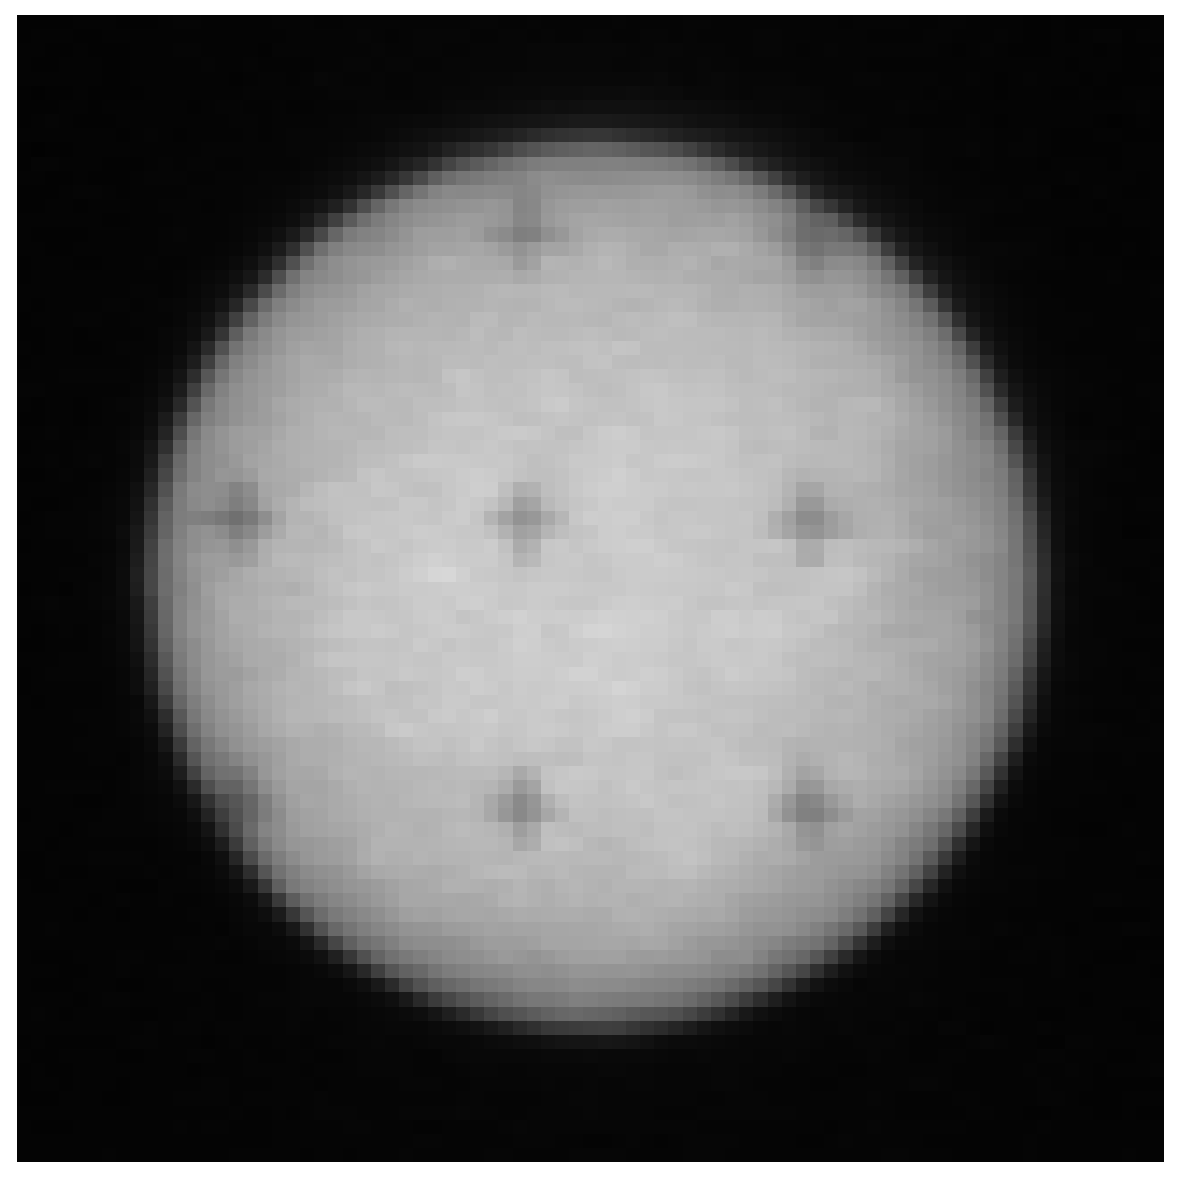
\includegraphics[width=.5\textwidth]{/Users/jerensuzuki/Documents/suncentering/orig_version/blurr.eps}
    \caption{Starting image}
    \label{image}
\end{figure}

\begin{figure}[!ht]
\ffigbox{
    \begin{subfloatrow}
        \ffigbox[\FBwidth]% Width of subfloat
        {
        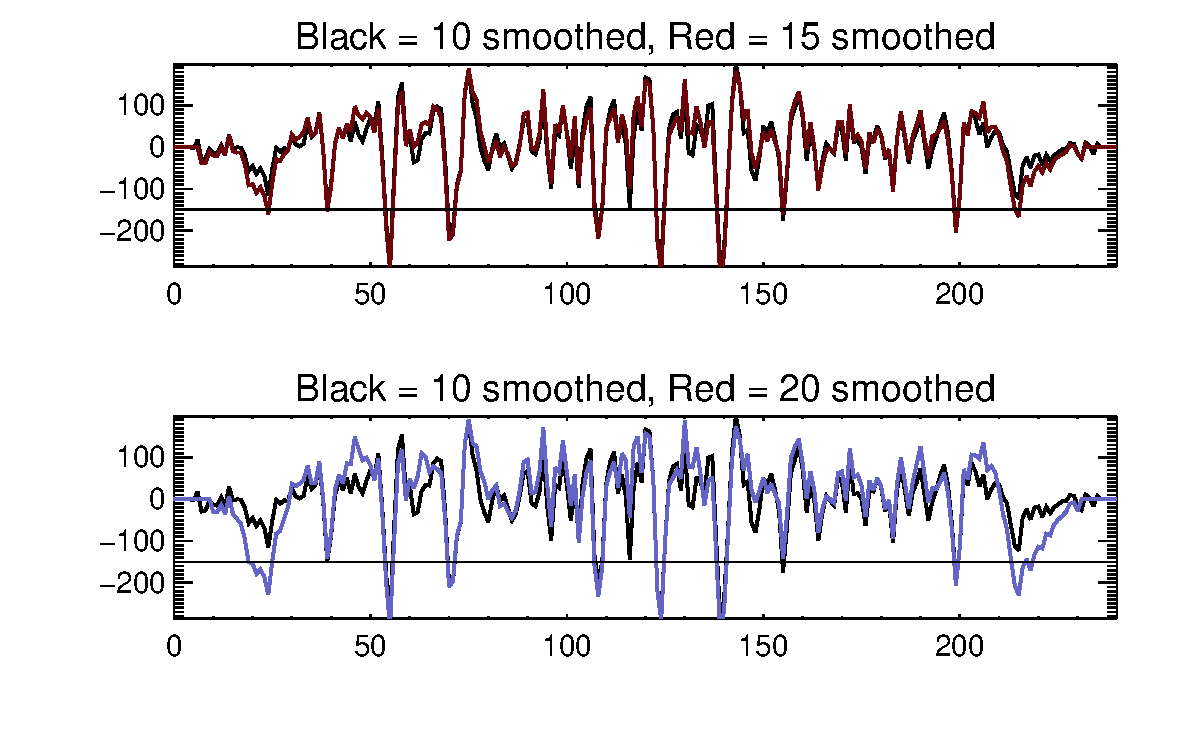
\includegraphics[width=.9\linewidth]{/Users/jerensuzuki/Documents/suncentering/orig_version/smoothcomp.eps}
        }
        {
        \subcaption{}
        \label{smoothed}
        }
    \end{subfloatrow}
    \begin{subfloatrow}
        \ffigbox[\FBwidth]% Width of subfloat
        {
        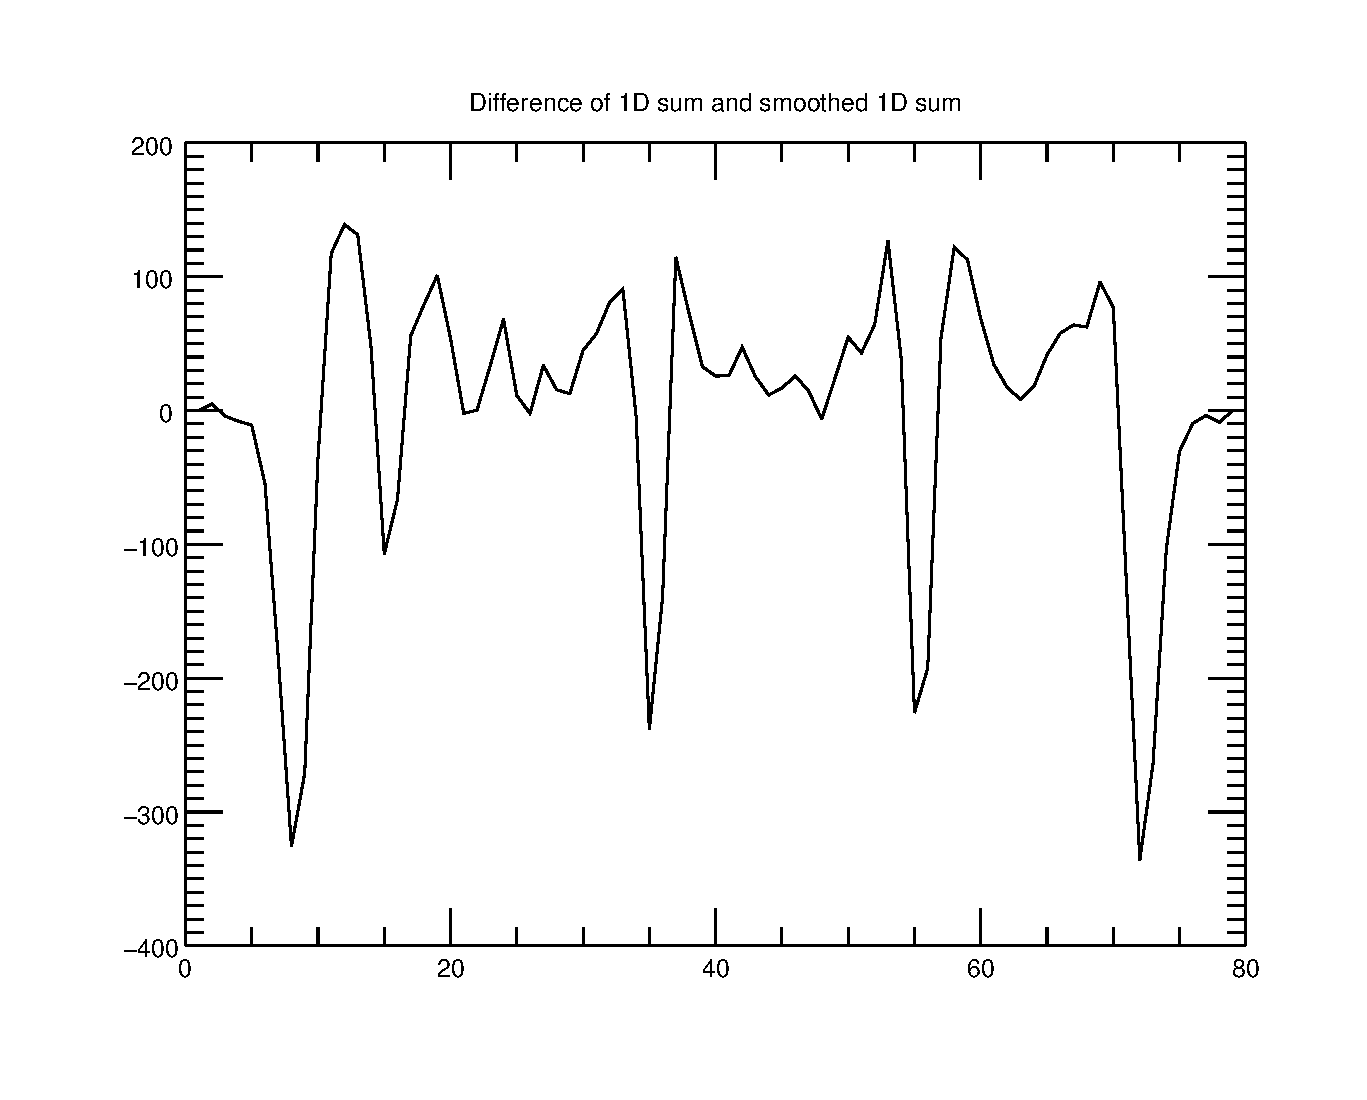
\includegraphics[width=.9\linewidth]{/Users/jerensuzuki/Documents/suncentering/orig_version/badpeaks.eps}
        }
        {
        \subcaption{}
        \label{sub}
        }
    \end{subfloatrow}
}
{
\caption{}
\label{colsums}
}
\end{figure}


Once we have the column and row postiions of our fiducials we go through each candidate and fall upon this fellow in Figure \ref{hidden}:

\begin{figure}[!ht]
    \centering
    \includegraphics[width=.5\textwidth]{/Users/jerensuzuki/Documents/suncentering/orig_version/hidden_fid.eps}
    \caption{Fiducial candidate}
    \label{hidden}
\end{figure}

We look at the column sum and get Figure \ref{colsum}. The line in red is the sum smoothed by 5 pixels. Subtracting the two gives us Figure \ref{drowned} and we can instantly see that the end of Figure \ref{colsum} is seriosuly messing up our peak detection. the peak should be around index 10 but according to Figure \ref{drowned}, it's at 4.

\begin{figure}[!ht]
\ffigbox{
    \begin{subfloatrow}
        \ffigbox[\FBwidth]% Width of subfloat
        {
        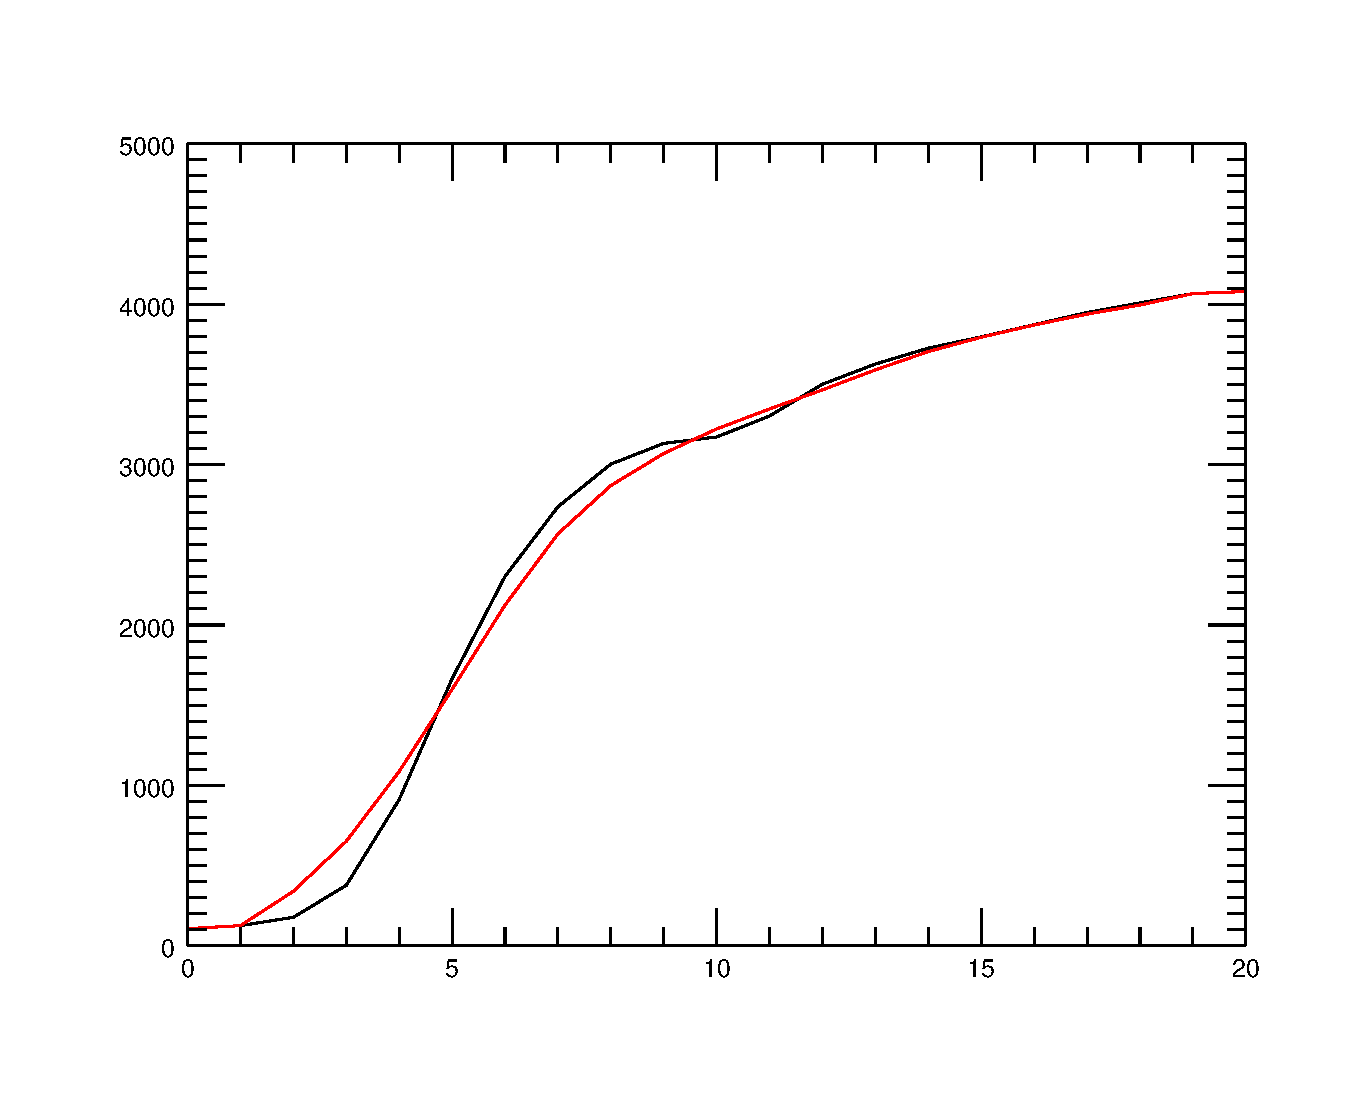
\includegraphics[width=.9\linewidth]{/Users/jerensuzuki/Documents/suncentering/orig_version/badsmooth.eps}
        }
        {
        \subcaption{}
        \label{colsum}
        }
    \end{subfloatrow}
    \begin{subfloatrow}
        \ffigbox[\FBwidth]% Width of subfloat
        {
        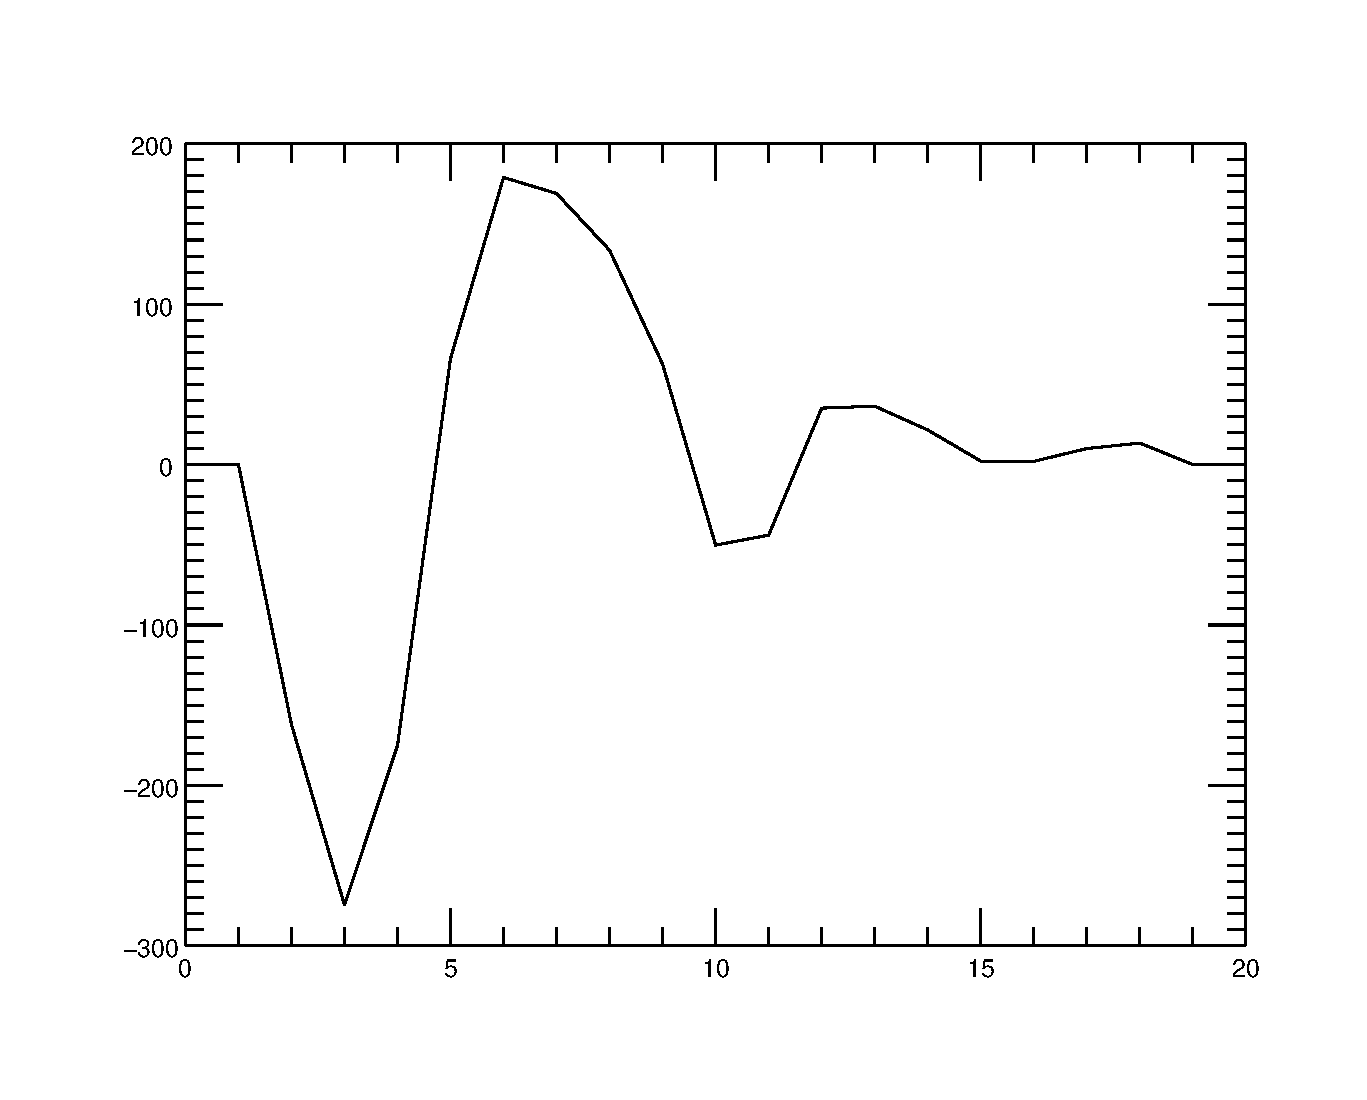
\includegraphics[width=.9\linewidth]{/Users/jerensuzuki/Documents/suncentering/orig_version/drowned.eps}
        }
        {
        \subcaption{}
        \label{drowned}
        }
    \end{subfloatrow}
}
{
\caption{}
\label{badfid}
}
\end{figure}

I tried looking at the column sum above 1000 and then smoothing but it didn't turn out that much better. I swear it worked before though. :(

\begin{figure}[!ht]
\ffigbox{
    \begin{subfloatrow}
        \ffigbox[\FBwidth]% Width of subfloat
        {
        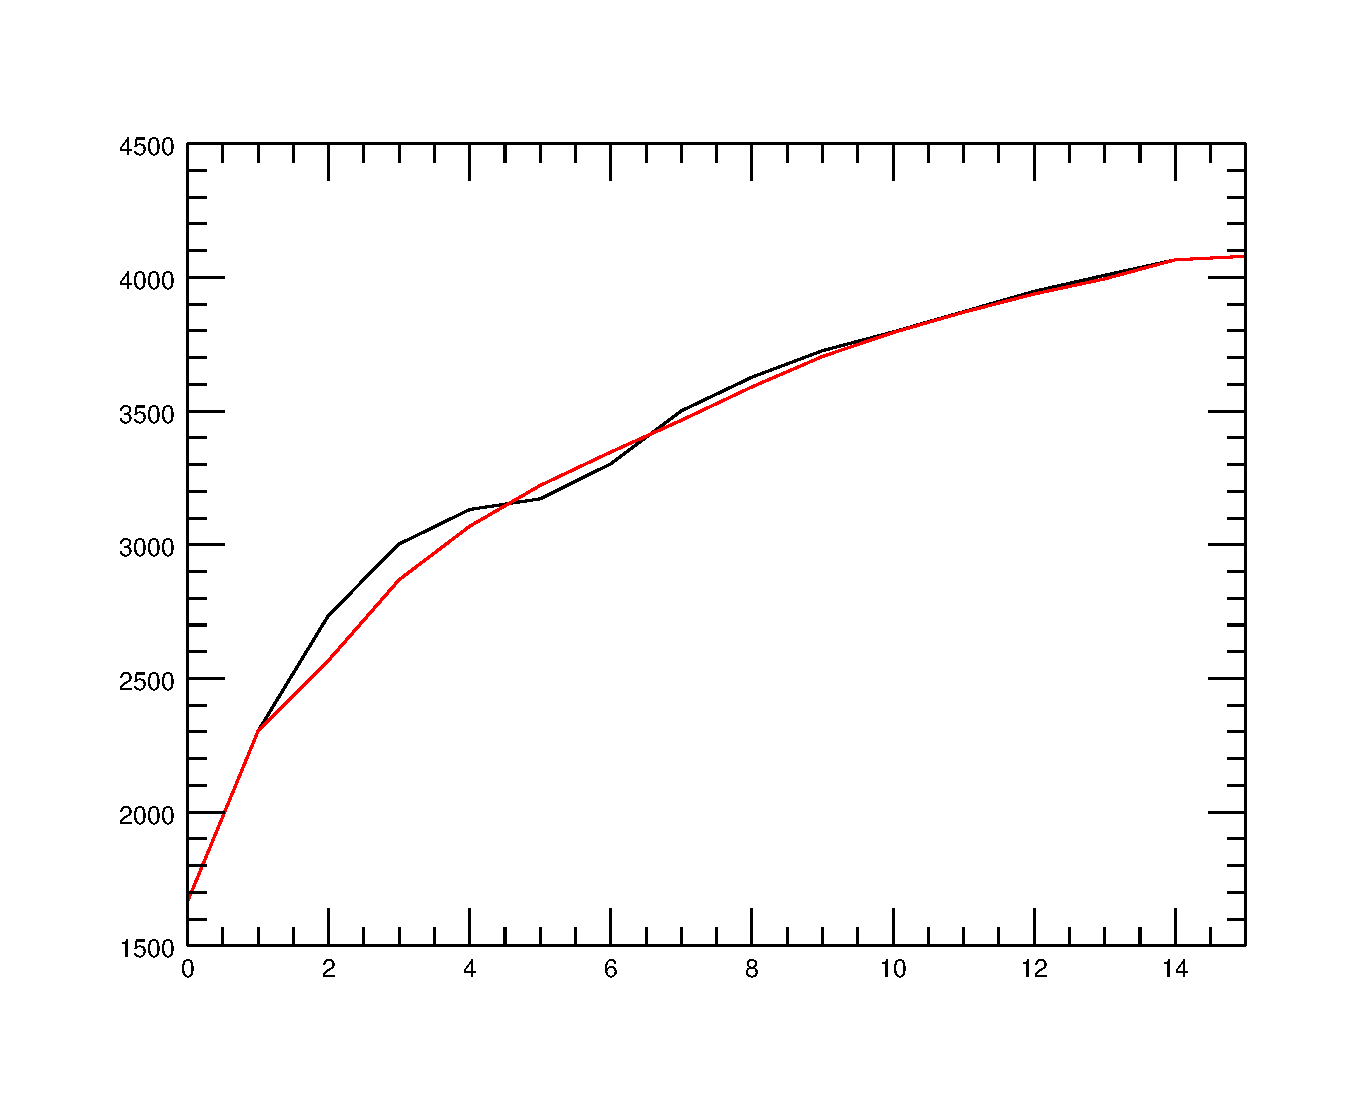
\includegraphics[width=.9\linewidth]{/Users/jerensuzuki/Documents/suncentering/orig_version/betterpeak.eps}
        }
        {
        \subcaption{}
        \label{betterpeak}
        }
    \end{subfloatrow}
    \begin{subfloatrow}
        \ffigbox[\FBwidth]% Width of subfloat
        {
        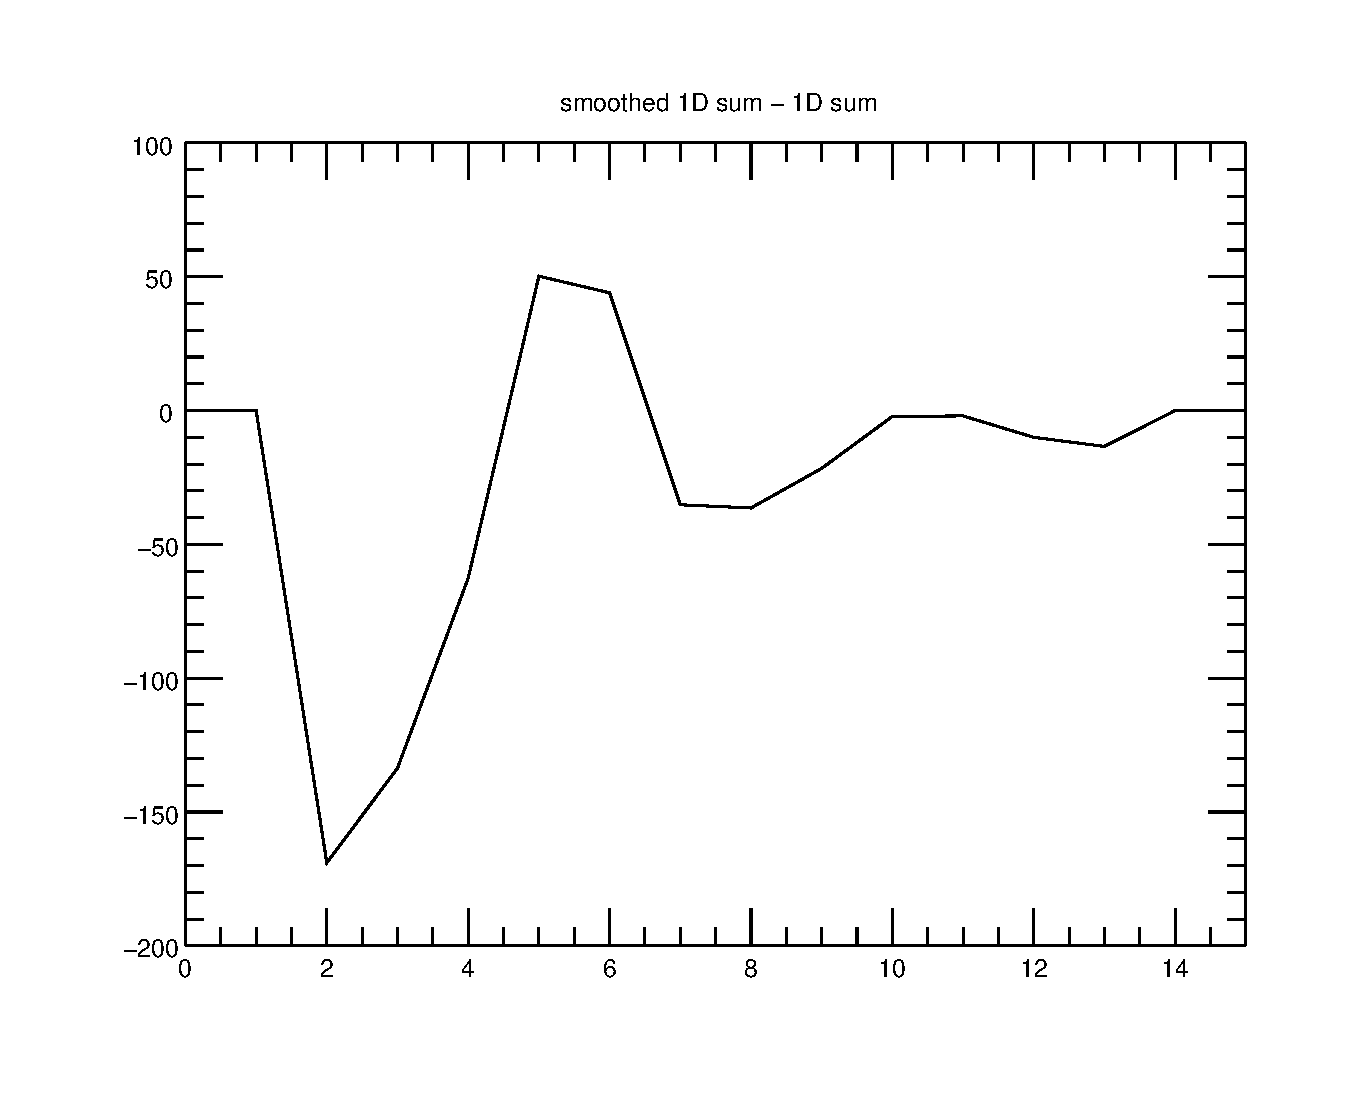
\includegraphics[width=.9\linewidth]{/Users/jerensuzuki/Documents/suncentering/orig_version/notbetter.eps}
        }
        {
        \subcaption{}
        \label{notbetter}
        }
    \end{subfloatrow}
}
{
\caption{}
\label{stillbadfid}
}
\end{figure}

% section First set of 1D smoothing (end)
\end{document}
